\graphicspath{{images/}}

\section{Determinante}

\begin{definition}{Geometrische Interpretation} der Determinante:\\
    \begin{minipage}{0.6\linewidth}
    \begin{itemize}
        \item Fläche im $\mathbb{R}^2$
        \item Volumen im $\mathbb{R}^3$
    \end{itemize}
    welche durch eine Matrix A aufgespannt wird.
    $$A = |\vec{a} \times \vec{b}| = |\det(A)|$$
    \end{minipage}
    \begin{minipage}{0.35\linewidth}
        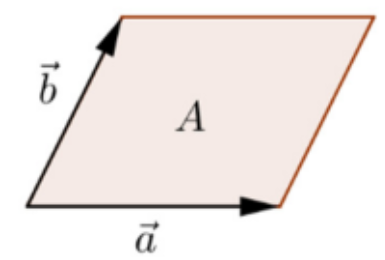
\includegraphics[width=0.9\linewidth]{determinante.png}
    \end{minipage}
\end{definition}

\begin{theorem}{Determinantenregeln}\\
    \begin{minipage}{0.5\linewidth}
        \begin{itemize}
            \item $\det(A) = \det(A^T)$
            \item $\det(A \cdot B) = \det(A) \cdot \det(B)$
            \item $\det(A^{-1}) = \frac{1}{\det(A)}$
        \end{itemize}
    \end{minipage}
    \begin{minipage}{0.5\linewidth}
        \begin{itemize}
            \item $\det(\lambda \cdot A) = \lambda^n \cdot \det(A)$
            \item $\det(A) = 0 \Leftrightarrow A$ ist singulär
        \end{itemize}
    \end{minipage}
\end{theorem}

\begin{formula}{Determinante einer $2 \times 2$-Matrix}
    $A = \begin{pmatrix} a & b \\ c & d \end{pmatrix}$
    \begin{itemize}
        \item $\det(A) = |A| = a \cdot d - b \cdot c$
    \end{itemize}
\end{formula}

\begin{formula}{Determinante einer $3 \times 3$-Matrix}
    $A = \begin{pmatrix} a & b & c \\ d & e & f \\ g & h & i \end{pmatrix}$\\
    \begin{minipage}{0.4\linewidth}
        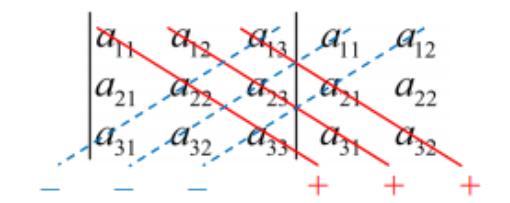
\includegraphics[width=0.8\linewidth]{determinante_3x3.png}
    \end{minipage}
    \begin{minipage}{0.5\linewidth}
        $|A| = a \cdot e \cdot i + b \cdot f \cdot g + c \cdot d \cdot h - c \cdot e \cdot g - b \cdot d \cdot i - a \cdot f \cdot h$
    \end{minipage}
\end{formula}

\begin{concept}{Determinante einer $ n \times n$-Matrix} $A$
    $$\det(A) = |A| = \sum_{j=1}^{n} (-1)^{i+j} \cdot a_{ij} \cdot |A_{ij}|$$
    \begin{itemize}
        \item Tipp: Entwickeln nach Spalte oder Zeile mit den meisten Nullen
        \item $|A_{ij}|$ ist die Determinante der $(n-1) \times (n-1)$-Matrix, die entsteht
    \end{itemize}
    evtl. bsp hier
\end{concept}

\begin{theorem}{Lineare Abhängigkeit}
    Die folgenden Aussagen sind äquivalent:
    \vspace*{2mm}
    \begin{itemize}
    \item $\operatorname{det}(A) \neq 0$
    \item Spalten von $A$ sind linear unabhängig
    \item Zeilen von $A$ sind linear unabhängig
    \item $r g(A)=n$
    \item $A$ ist invertierbar
    \item Das LGS $A \cdot \vec{x}=\vec{c}$ hat eine eindeutige Lösung
    \end{itemize}
\end{theorem}

